\chapter{Results}

\section{example situation 1}

You are a scientist involved with the MIKE Programm (Monitoring the Illegal Killing of Elephants). Your object of investigation is to find covariates for the intensity of illegally killed elephants in Africa. You have access to data collected within the Great Elephant Census, a continent-wide aerial survey counting the number and distribution of elephants within there territories. 
Image X shows the study area, each region corresponds to a territory and for each territory, you have the aggregated number of illegally killed elephants. To run your statistical model in R and find influential covariates you need further environmental variables derived from satellite imagery like the topography, land-use, precipitation et cetera. 
Although the study area is fragmented and of large-scale at the same time to acquire the data with the GEE2R package is pretty convenient.
The study area is fragmented and of large-scale at the same time. 
data product
After installing the GEE2R package the first step is to initialize the package with \texttt{ee\_grab\_init()}. As described in the section (methods dependencies) the function installs all additionally required dependencies and guides the user through the authentication processes to activate the different API's. To authenticate to the API the user has to log in to his Google account and allow the API to access data on googles servers on the user's behalf. If the Google account is verified and the permission is granted, the user is directed to an authentification token. This token is manually copied and pasted into a running command line script, which creates persistent credentials. 
Later, the credentials are used to authenticate a request to the API. To simplify this procedure the \texttt{ee\_grab\_init()} function successively opens a browser window to log into the Google account and a corresponding command line window to enter the token. This process is repeated for each API. If the function runs successfully, all needed credentials are stored for further sessions. Because some of the credentials expire after a few hours, a reauthentication is necessary. This process is handled automatically inside the \texttt{ee\_grab()} function. If a reauthentication is needed the function opens a browser window and the user is asked to log in with his google account, the creation of credentials is automated and there is no need to copy or paste the token manually.
To acquire the data next the \texttt{ee\_grab()} function is used.

\begin{center}

	\begin{figure}[h]
		\begin{center}
			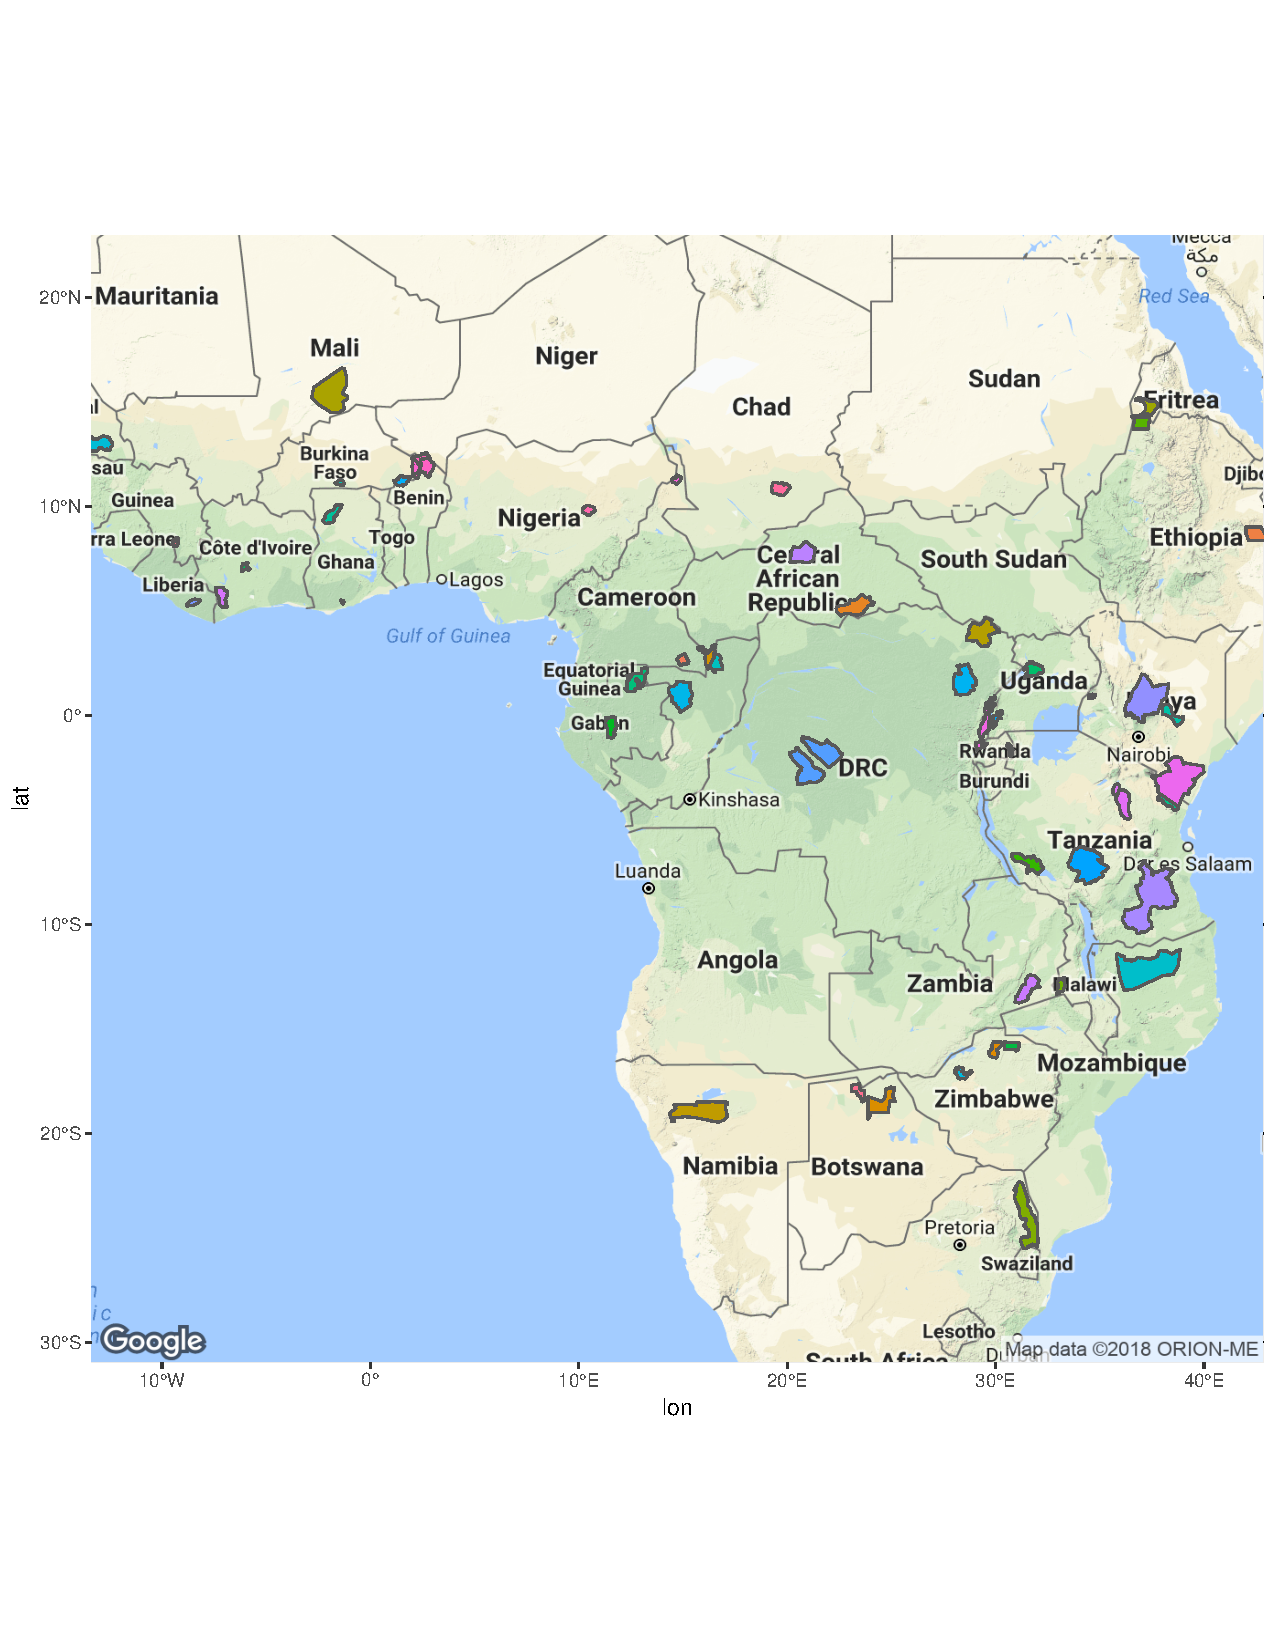
\includegraphics[width=15cm]{images/territories.pdf}
		\end{center}
	\end{figure}
	% \vskip 2em%
\end{center}

The target is the path to the shapefile of the elephant territories shown in image X. The products argument takes a list of earth engine data product-functions. Each function specifies one particular data product and it's necessary parameter. The name of the function is \texttt{eeProduct\_ }followed by the source of the data products, underscore the name of the data product. For example: \texttt{eeProduct\_modis\_treecover()}. The output of the function is simply an Object of class list, that specifies the parameters of the requested data product. To use a function, that produces the required parameters instead of committing a list or a vector with the listed parameter, holds several advantages. Because all data products start with \texttt{eeProduct\_ }, by simply typing \texttt{eeProduct\_ }, R's autocomplete function opens a drop-down menu of all available data products. Furthermore, the selection of a product in the menu displays a little description of the product and list their possible parameters. For more Information on a particular data product simply open the documentation of the function by pressing F1, or use equivalent methods. This way, it's possible to browse through the products, without any additional metadata outside of R. Additionally the functions provide default parameter values, that allow a test run without the need of specifying any parameter. While this procedure provides a user-friendly selection of available data products with their corresponding parameters it also minimises potential typing and spelling errors.
After browsing through the data products you choose the modis-tree-cover product for the year 2000 to 2005. You are further interested in the mean tree cover between this period and also want the mean tree cover in each of your territories. Because the default value for the time reducer and the spatial reducer is mean you only need to specify the time interval parameter with a vector of the start and end-year (\texttt{timeInterval = c(2000, 2005)}). You are further interested in a potential correlation of the accessibility to populated areas and the illegally killed elephant, therefore you additionally choose the oxford-accessibility product. The information displayed by the R's autocompleting feature reveals only one possible parameter - spatialReducer - and by requesting the documentation of the function you learn that this data product is only available for the year 2015, and therefore has no temporal resolution to aggregate. Again, you choose the mean accessibility in each territory by using the default value of the parameter and add the function product to the list. The last argument specifies is the resolution in meters (edge length). The resolution sets the resolution of the processed data in Earth Engine and applies for all products. A value smaller than the native resolution of the data product results in Earth Engine resampling the data with the default nearest neighbour method, values higher result in a pixel aggregation with a default method mean. In the documentation, you learned that the native resolution of the tree cover product is 250m while the accessibility products provide a resolution of 30m. Because the area of the territories is of large-scale (mean area of the territories is 9862 square kilometres) you choose 1000m as the scale of your analysis. The resolution parameter strongly controls the scope of computation and out of this the processing time, therefore it's a good choice to not unnecessarily set him too low. 
Since all parameters are set, the function can be executed. 

\begin{lstlisting}
library(earthEngineGrabR)

ee_grab_init()


africa_elephant_data <- ee_grab(
target = "../Data/drought_sites/mike_bnd_af.shp",
products = list(
eeProduct_modis_treeCover(yearIntervall = c(2008, 2012)),
eeProduct_oxford_accessibility()
),
resolution = 1000
)
\end{lstlisting}


As most processes of the function call are processed on googles servers, the execution time depends strongly on the throughput of your analysis on the servers and only slightly on the performance of your local machine. However, because of the upload and download process during the function execution, very low internet speed (1 Mbit/s in download and 0.1 Mbit/s in upload) can work as a bottleneck, particularly during the upload process. 
On a 64 bit ubuntu machine with 8 Gbit RAM, 4 cores with 2.40GHz and internet speed of $10 \frac{Mbit}{s}$ in download and $1 \frac{Mbit}{s}$ in upload the \texttt{ee\_grab } function took 55 seconds to execute. All further time measurements refer to this setting.
The output of the \texttt{ee\_grab} function is an object of class "sf". The "sf" package provides a convenient approach to work with vector data in R and tries to succeed the widely used "sp" package in the future. For further information about the "sf" package see (). An "sf" object is basically a data.frame with an additional geometry list-column, what strongly simplifies manipulating an "sf" object by filtering, selecting or summarising.  The output of the \texttt{ee\_grab} function always contains all properties of the original target with the added products. The object new produced columns for the data products and a geometry column (see table X).


\begin{center}
	
	\begin{figure}[h]
		\begin{center}
			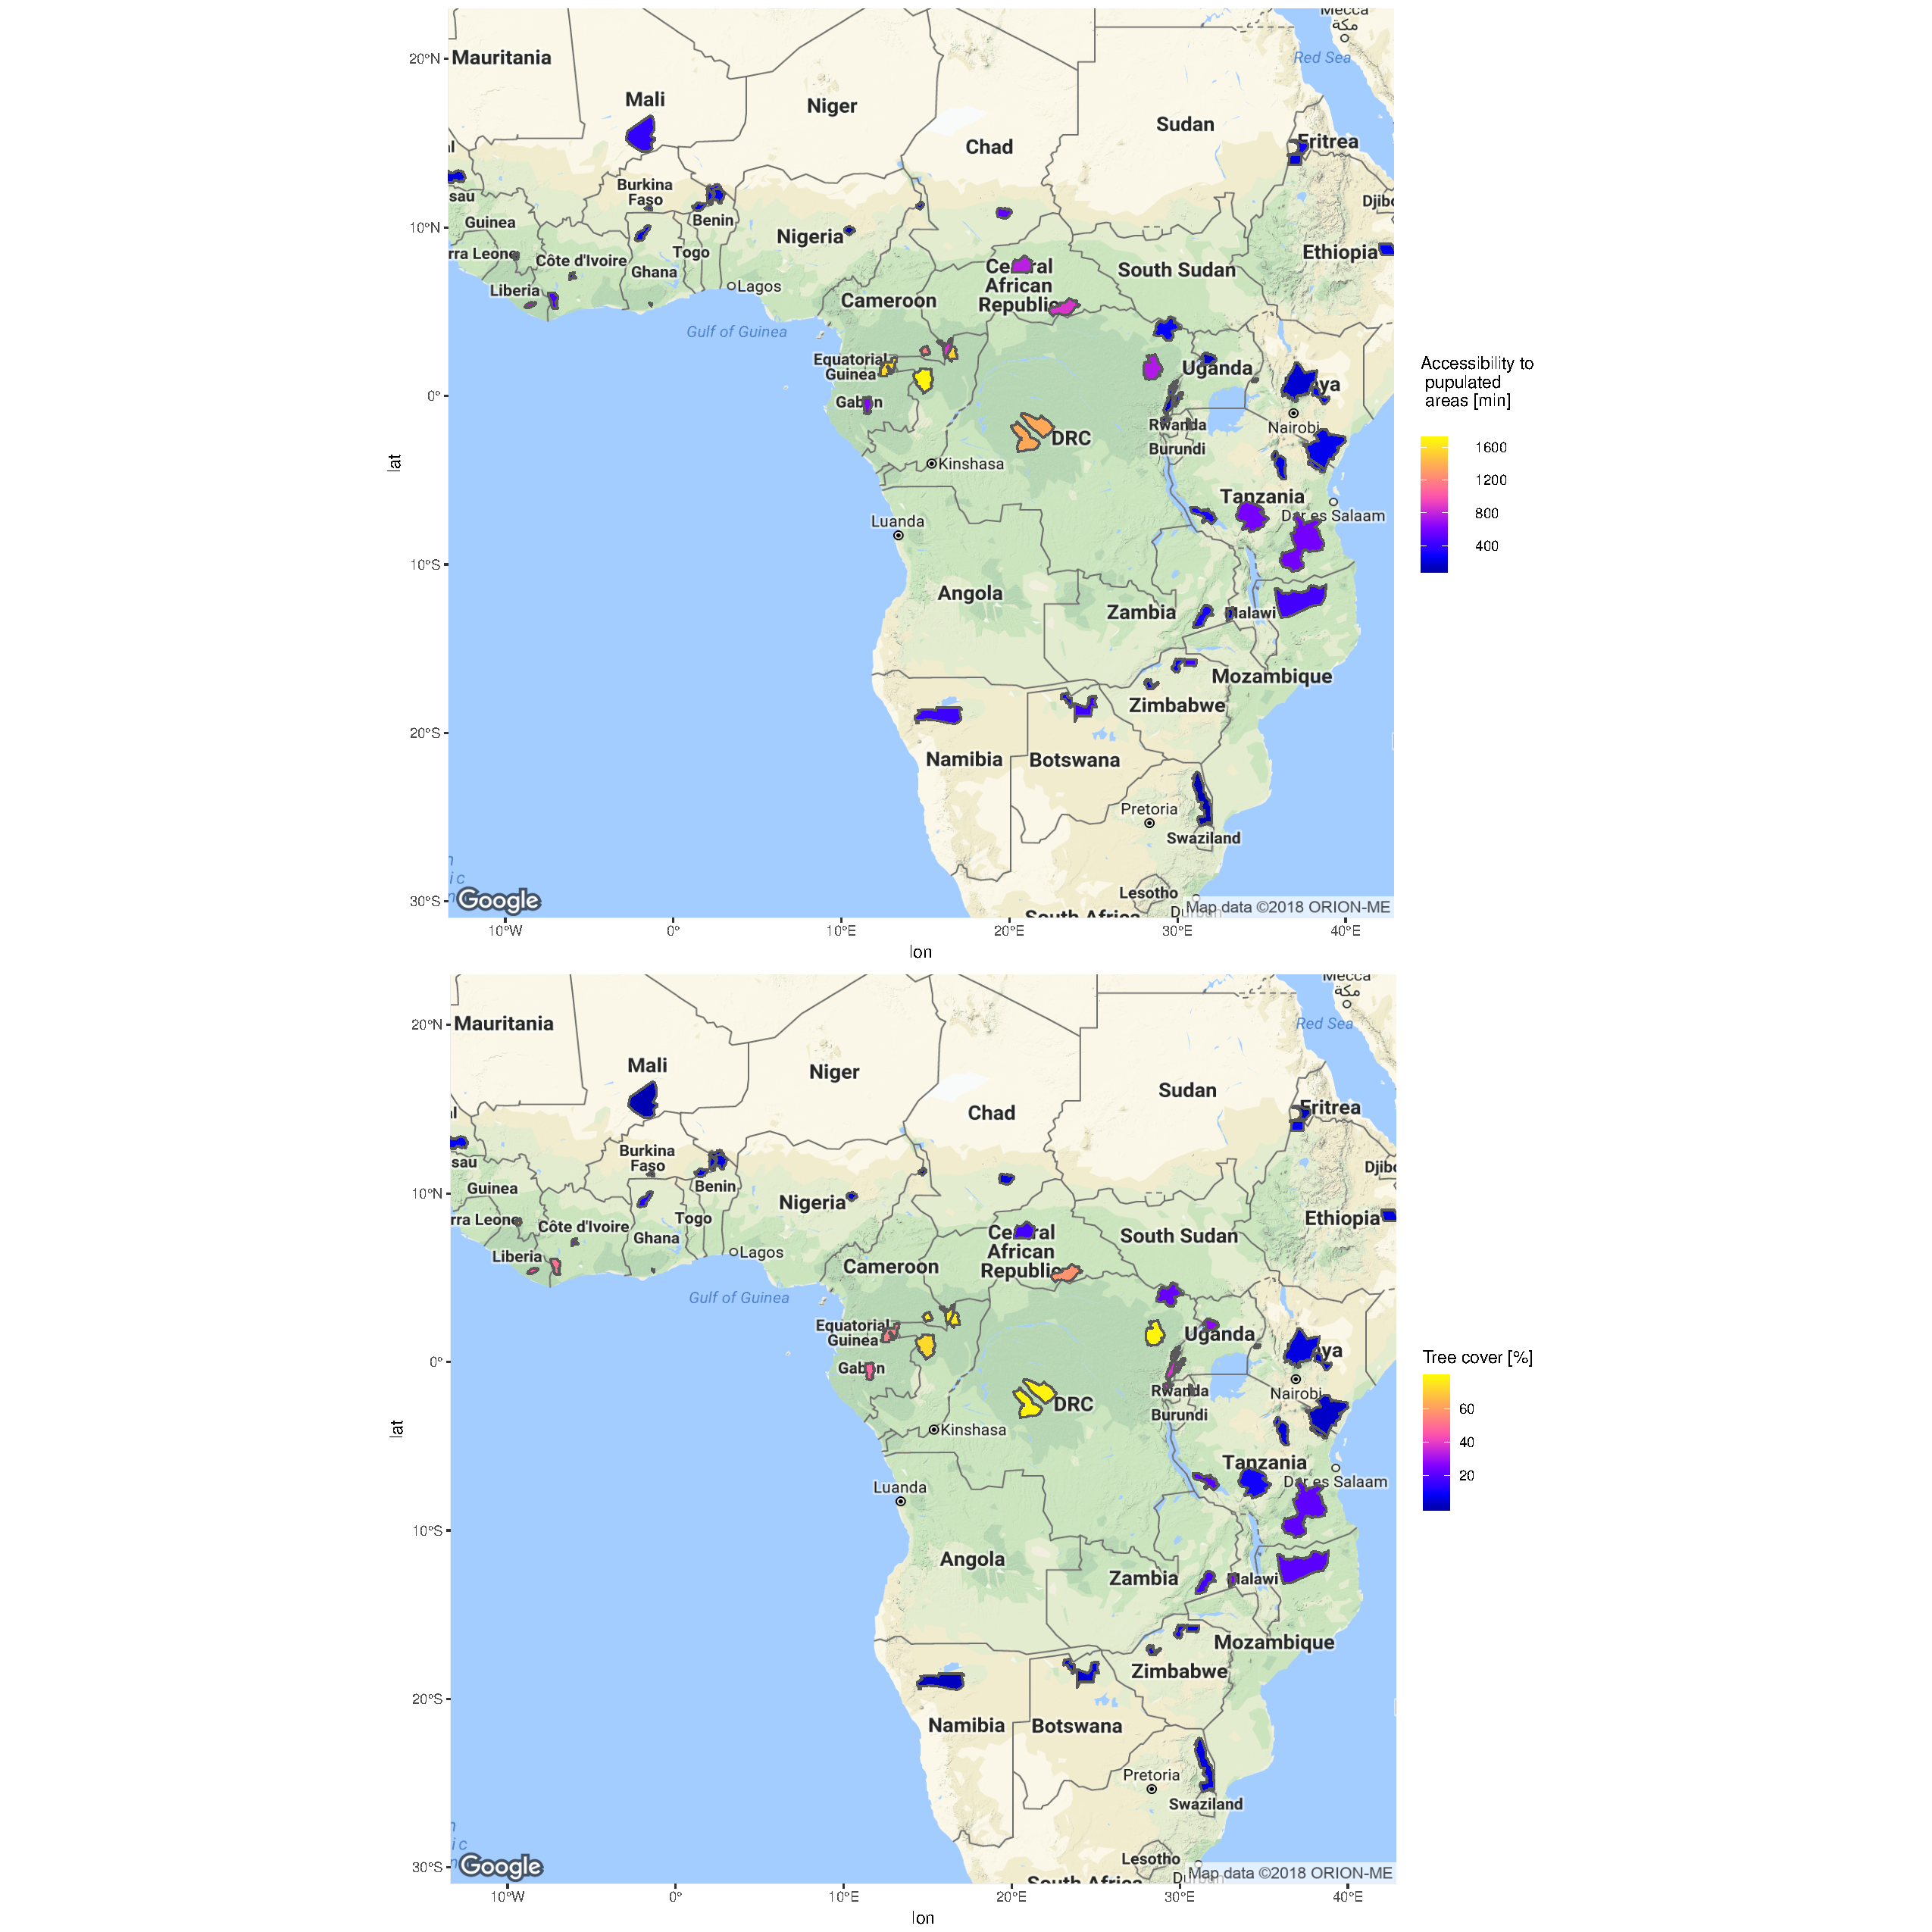
\includegraphics[width=15cm]{images/sample_session_1.pdf}
		\end{center}
	\end{figure}
	% \vskip 2em%
\end{center}

Map X shows the two data products. Eye-catching but not surprising is the negative correlation between accessibility and tree cover resulting in a regional pattern with the highest tree cover and lowest accessibility found in central Africa, while toward the north, south and west, the accessibility increases and the tree cover decreases.

While this sample session shows the capabilities of the earthEngineGrabR package to aggregate over large areas, the next example is dedicated to the opposite situation. 


\section{sample session 2}
\tableofcontents
let's stay with the invented scientist and his situation already described. Because of your access to the Great Elephant Census data you not only have the aggregated data for each territory but also the pre-aggregated survey data consisting of the number of elephants counted within a region specified by position, hight and the flight path of the aircraft. The combined regions form the spatial coverage of the survey and are available as shapefiles.

\begin{center}
	
	\begin{figure}[h]
		\begin{center}
			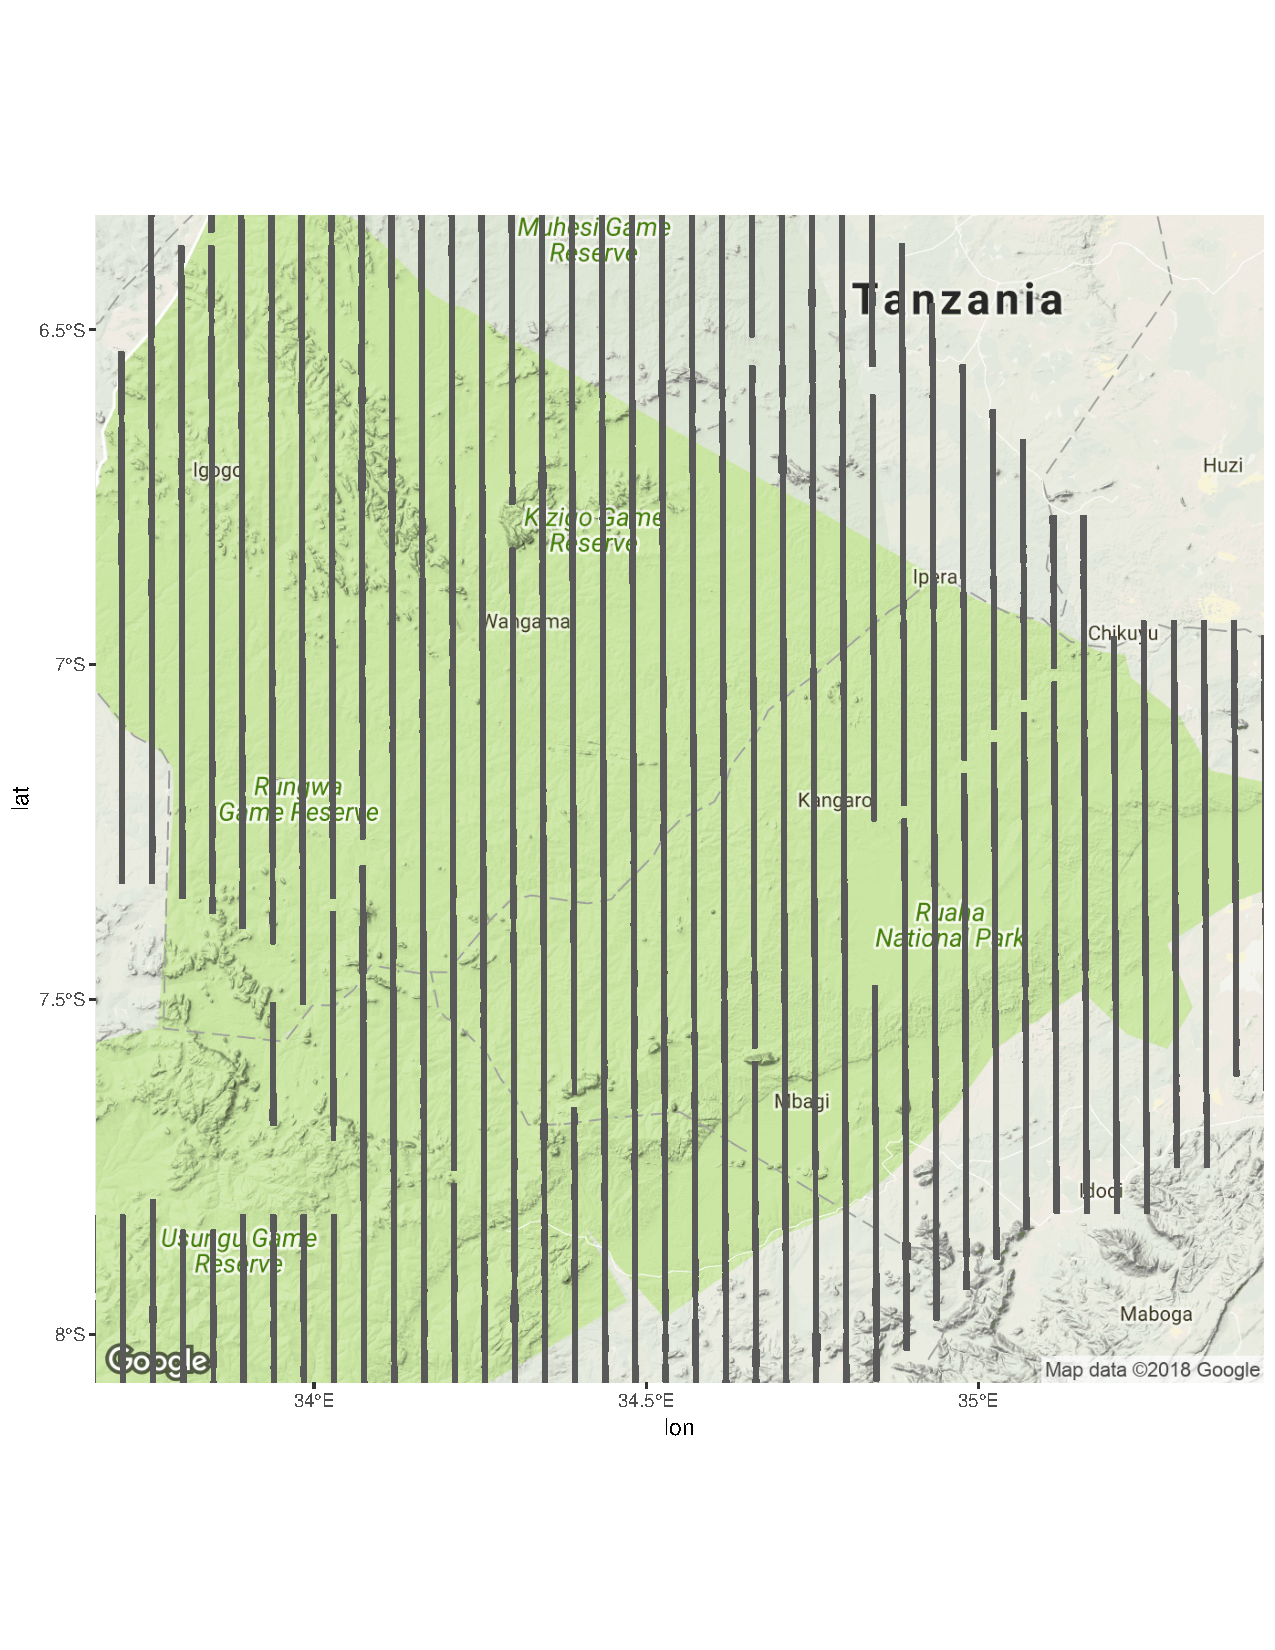
\includegraphics[width=15cm]{images/stripes.pdf}
		\end{center}
	\end{figure}
	% \vskip 2em%
\end{center}


Map X shows the coverage for Tanzania. This time you are interested in the availability of surface water in each of these regions, therefore you want to use the distance to surface water data product available in the earthEngineGrabR package. As the target, you use the shapefile of the survey coverage and only specify the \texttt{jrc\_distanceToWater} product in the products argument. As spatial and temporal reducer you choose median. 

\begin{lstlisting}

africa_elephant_data_stripes <- ee_grab(
target = "../Data/Strips_shapefiles/RR16StripsAlignedForFig.shp", 
products = list(
eeProduct_jrc_distanceToWater(yearIntervall = c(2000,2000), spatialReducer = "median")
),
resolution = 100
)
\end{lstlisting}




Due to the smaller area of the features of the target (mean area of 0.7 square kilometre), you choose a resolution of 50 meters and execute the function. The computation time takes about 3 minutes and the result is shown in map .y Since the area of the coverage is too small for a meaningful visualisation, map X shows a strongly zoomed view of the actual map x. 

\begin{center}
	
	\begin{figure}[h]
		\begin{center}
			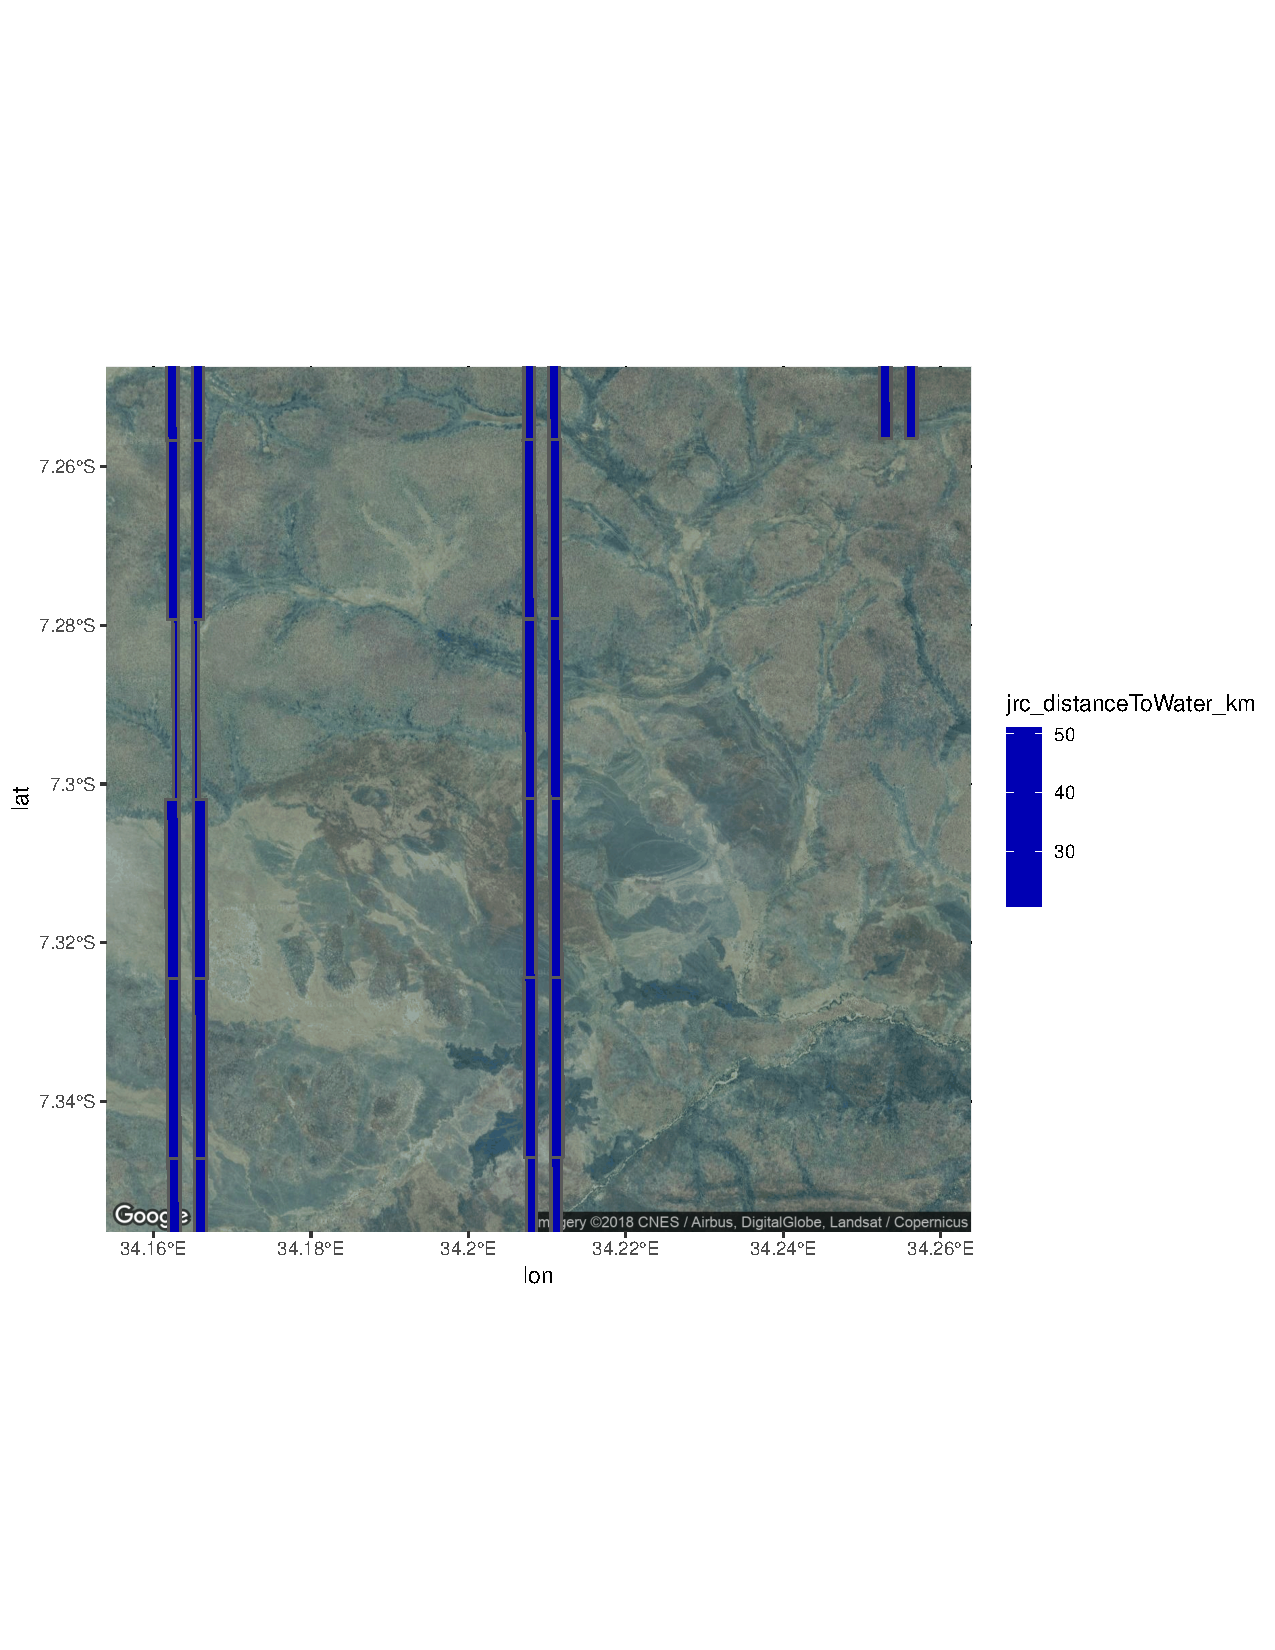
\includegraphics[width=15cm]{images/stripes_distance_zoom.pdf}
		\end{center}
	\end{figure}
	% \vskip 2em%
\end{center}



This example shows the flexibility of the earthEngineGrabR referred to the scale of analysis and the shape of the target.

In the last example, a more extended use case of the \texttt{ee\_grab} function is presented.


\section{sample session 3}

As a scientist, you are also interested in changes over time, for example, the change of precipitation in the elephant territories. Out of the documentation you know, that the precipitation product of the earthEngineGrabR is available from 2000 to 2015 on a yearly basis, thus you decide to calculate the precipitation for each year from 2000 to 2015 and analyse the change by using a linear model. The chirps precipitation product is produced from satellite data on a daily basis, what offers the possibility to calculate the yearly precipitation sum. Because the yearly precipitation sum is a common practice in hydrology and compared to the mean not this prone to extreme values you decide to calculate the yearly sum in each of the elephant territories for each year. To achieve that, you simply use the \texttt{ee\_grab} function, iterate over each year and collect the iteration products as follows:

\begin{lstlisting}

years <- 2000:2015
# empty data.frame for iteration
precipitation_all_years <- data.frame("name" <- NULL,"chirps_precipitation_mm" <- NULL, "year" <- NULL)

for (i in years) {
# to inform
cut(paste("processing of year:", i))
# grab precipitation for year = i
precipitation_year <- ee_grab(
target = "../Data/drought_sites/mike_bnd_af.shp",
products = list(
eeProduct_chirps_precipitation(yearIntervall = c(i, i), temporalReducer = "sum")
),
resolution = 1000
)
# to drop geometry, select variables of interest and creat a year column
precipitation_year_clean <- precipitation_year %>% 
sf::st_set_geometry(NULL) %>% 
dplyr::select(chirps_precipitation_mm, name) %>% 
dplyr::mutate(year = i)
# accumulate iteration products
precipitation_all_years <- dplyr::bind_rows(precipitation_all_years, precipitation_year_clean)
}
\end{lstlisting}




As temporal reducer, you choose sum, for the year interval, you take the i-th value of the created years vector. Due to the large-scale of your analysis, you again choose a resolution of 1000 meters. Since you want the spatial mean of the yearly precipitation sum in the territories, which already is the default spatial reducer, all necessary parameters in the \texttt{ee\_grab} function are specified. While the processing of a single request for one year would take about 3 minutes, the processing time of the entire for loop is only about 15 minutes. Because the requests are sent and processed in parallel, the relationship of the processing time and the number of requests is nonlinear. This point will be explained further in the discussion. The output of this loop is data.frame with a column for the sum of precipitation, year and name of the territory.  To quickly calculate, a linear model of the sum of precipitation explained by year for each of the territories you use a combination of functions from the dplyr and broom R packages. With dplyr's \texttt{group\_by} and do function you calculate a linear model for each of the territories and with the tidy function from broom and some selecting and filtering you extract the wanted estimates. The estimates show the linear effect of year on the yearly precipitation sum for each of the territories. 
By joining the estimates with the spatial data of the territories the estimates can be visualised spatially. 

\begin{center}
	\begin{figure}[h]
		\begin{center}
			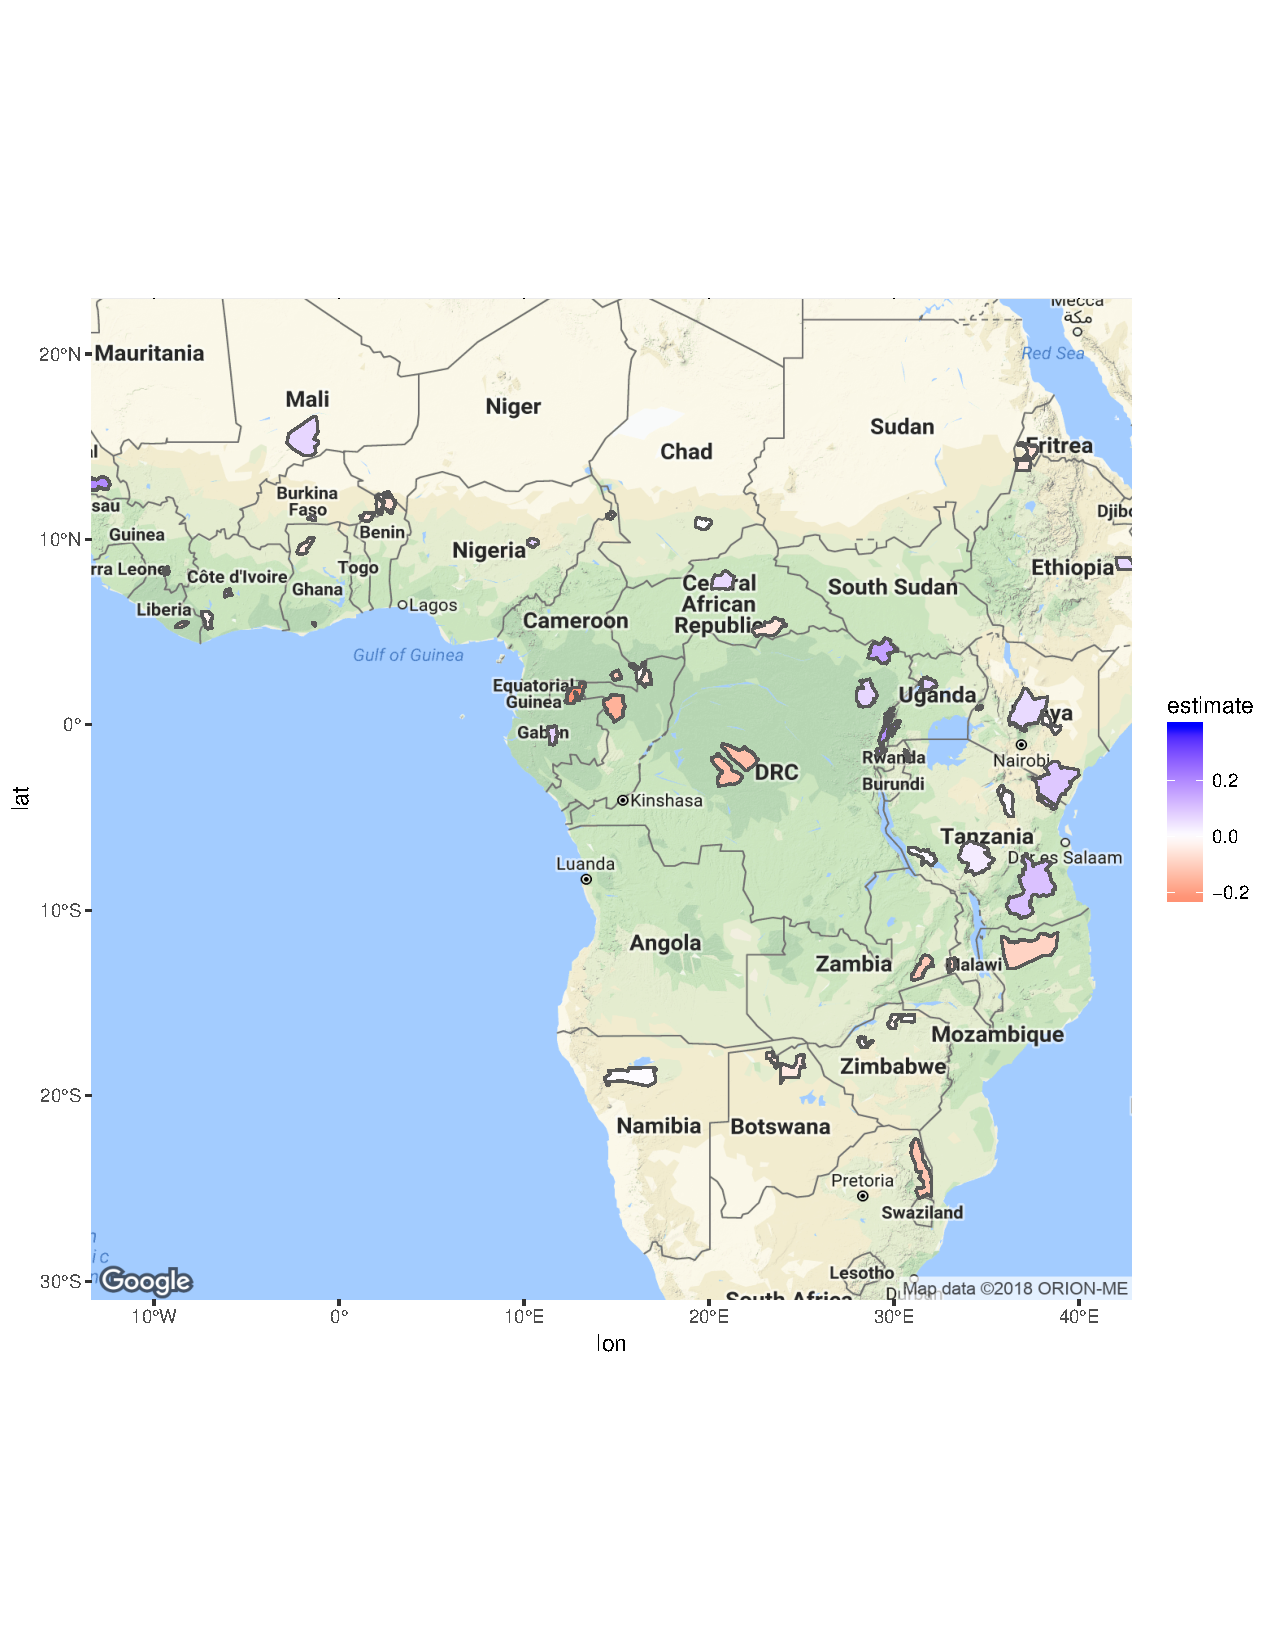
\includegraphics[width=15cm]{images/sample_session_3_change_map.pdf}
		\end{center}
	\end{figure}
	% \vskip 2em%
\end{center}



MapX shows the estimate of the yearly change of the yearly precipitation sum in for each territory. Given, that those estimates reflect a yearly change some values are remarkable hight. While the yearly precipitation sum is increasing for the territories in East Africa, it is decreasing for most territories in central Africa, especially for those with hight tree cover (see map X).

